\chapter{The XPS Method}\label{ch:xps}
X-ray induced Photoelectron Spectroscopy (XPS) relies on a well know principle namely the photo-electric effect, which was explained by Einstein in 1905. When a surface is bombarded with photons with sufficient energy an electron may adsorb all the energy of the photon and be able to escape the solid with a kinetic energy reflecting the photon energy as well as the bonding energy of the electron. It was not until in the late sixties that this process was brought into operation by Kai Siegbahn who later received the Nobel prize for his work. The process is illustrated in \autoref{fig:photoemission}

\begin{figure}[h!]
	\begin{center}
	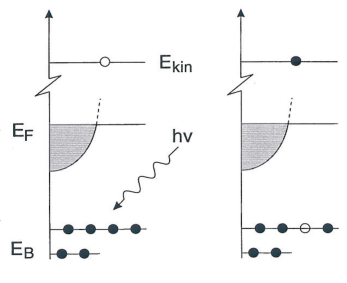
\includegraphics[scale=3]{figures/04_01.png}
	\caption{Sketch of the photoemission process.}
	\label{fig:photoemission}
	\end{center}
\end{figure}

X-rays are generated with a suitable  energy so that the electrons, excited from the atoms, have a kinetic energy in  the range where high surface sensitivity can be obtained. The kinetic energy of the emitted electron relative to the vacuum level will be given by

\begin{equation}
E_{kin}=h\nu-E_B-\Phi
\end{equation}

\noindent where h$\nu$ is the photon energy of the X-ray, $E_B$ is the binding energy of the electron in the solid referred to the Fermi level, and $\Phi$ is the work  function for the solid. It is obvious that if we can generate a monochromatic source of X-rays it is possible to map out the electron density as a function of binding energy by measuring the kinetic energy of the emitted electrons. Since the electron density as a function of binding energy is characteristic for each element this is a useful method to determine not only which elements are present in the surface but also how much there is  of each. Furthermore, small shifts in the measured binding energy  reflect changes of the chemical state of the elements. The XPS method has therefore also been called Electron Spectroscopy for Chemical Analysis (ESCA).

\section{X-ray Sources}
When a material is bombarded with electrons there will, as we saw in Chapter \ref{ch:reqs}, be possibilities for ionisation of the atoms in the material. The excited atom will after a very short time relax by a process where a weakly bound electron is dropping down into the created vacancy. The energy released by this process can now be used to either excite another bound electron out of the atom (an Auger process) or in this case more interesting to emit a photon. In \autoref{fig:dualanode} a dual anode is shown which is bombarded with \SI{15}{k\electronvolt} electrons.

\begin{figure}[h!]
	\begin{center}
	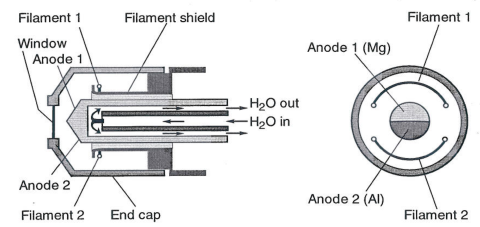
\includegraphics[scale=3]{figures/04_02.png}
	\caption{Schematics of a commercial dual
          X-ray anode.}
	\label{fig:dualanode}
	\end{center}
\end{figure}

A thin aluminium foil is mounted just in front of the anode in order to prevent stray electrons and outgassing to the rest of the chamber.

The process is shown for an aluminium atom in \autoref{fig:altransition}. Initially a hole is formed in the 1s level. The atom may now relax by either letting an electron  from the 2p$_{\frac{3}{2}}$ or 2p$_{\frac{1}{2}}$ fall down and emit a photon. The energy splitting between the two p levels  is due to spin-orbit coupling and is very small (\SIrange{0.4}{0.5}{\electronvolt}).

\begin{figure}[h!]
	\begin{center}
	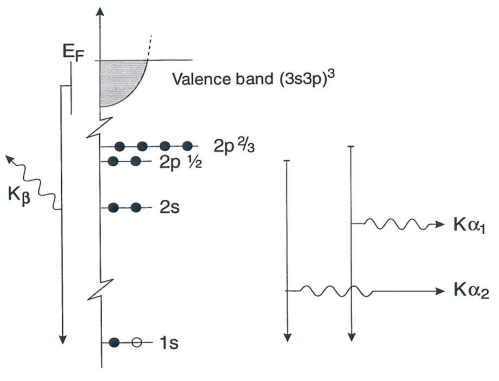
\includegraphics[scale=3]{figures/04_03.png}
	\caption{Sketch of the transitions in
          aluminium leading to the Al$_{K\alpha}$ radiation.}
	\label{fig:altransition}
	\end{center}
\end{figure}

Unfortunately, the short lifetime of the excited states involved will also influence the widths of the emitted X-rays. The relations are given through the Heisenberg uncertainty relation for energy and time

\begin{equation}
\Delta E \Delta t \geq \frac{h}{2\pi}
\end{equation}

\noindent and leads to, as shown in \autoref{fig:albroadening}, a broadening of \SI{0.7}{\electronvolt} for each of the two lines \cite{siegbahn1}. Thus the X-ray emitted by this transition will effectively be one line which will be roughly \SI{1.0}{\electronvolt} broad at Full Width Half Maximum (FWHM) with an energy of \SI{1486.6}{\electronvolt}.

\begin{figure}[h!]
	\begin{center}
	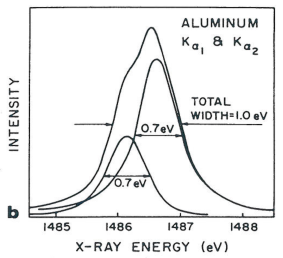
\includegraphics[scale=4]{figures/04_04.png}
	\caption{The line width of the $K_{\alpha 1}$ and $K_{\alpha2}$ resulting in the $K_{\alpha 12}$ line \cite{siegbahn1}.}
	\label{fig:albroadening}
	\end{center}
\end{figure}

Due to an old X-ray notation this transition is called an Al$_{K_{\alpha 12}}$ line indicating that a hole is generated in the $K$ shell (main quantum number one i.e. 1s). A quite similar transition exists in magnesium which is a bit more narrow (\SI{0.7}{\electronvolt}) and has an energy of \SI{1253.6}{\electronvolt}. Many other materials may be used as anodes as shown in Table \ref{tab:transenergies}, but in general Mg and Al are the preferred species to have on a dual anode as shown in \autoref{fig:dualanode}.

\begin{table}
\begin{center}
\caption{Energies and FWHMs of various X-ray transitions.}\label{tab:transenergies}
\begin{tabular}{|l|r|r|} \hline
X-ray line & Energy [\si{\electronvolt}] & FWHM [\si{\electronvolt}] \\ \hline
Mg$_{K_{\alpha}}$ & 1253.6 & 0.70 \\ \hline
Al$_{K_{\alpha}}$ & 1486.6 & 0.85 \\ \hline
Si$_{K_{\alpha}}$ & 1739.5 & 1.2 \\ \hline
Zr$_{L_{\alpha}}$ & 2042.4 & 0.77 \\ \hline
Ag$_{L_{\alpha}}$ & 2984 & $<3$ \\ \hline
Ti$_{L_{\alpha}}$ & 4511 & 1.4 \\ \hline
Cr$_{L_{\alpha}}$ & 5414.7 & 1.8 \\ \hline
Cu$_{L_{\alpha}}$ & 8048 & 2.5 \\ \hline
\end{tabular}
\end{center}
\end{table}

The reason being that a narrow line is desired in combination with sufficient energy in order to be able to reach several core levels in the sample material.

Usually the Al$_{K_{\alpha 12}}$ and Mg$_{K_{\alpha 12}}$ are sufficient for most purposes, but when detailed studies are necessary it is important to consider the quality of the X-ray source as there will be other possibilities for transitions in the anode. \autoref{fig:highenergybomb} shows the number of photons emitted from an aluminium anode as a function of photon energy when it is bombarded with $E_p=\SI{15}{k\electronvolt}$ electrons schematically.

\begin{figure}[h!]
	\begin{center}
	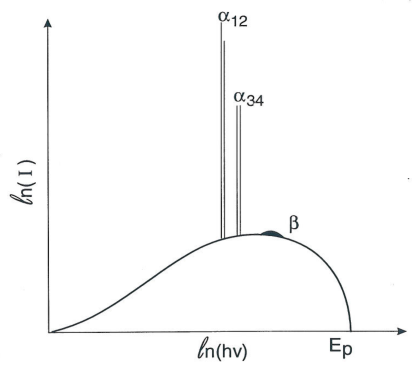
\includegraphics[scale=3.5]{figures/04_05.png}
	\caption{Sketch of the X-ray emission spectrum for an anode bombarded with high energy ($E_p$) electrons.}
	\label{fig:highenergybomb}
	\end{center}
\end{figure}

There will be a continuously weak background of photons due to the deceleration of the electrons in the anode. Besides this there is a strong and a discrete contribution from the 1s-2p transition as discussed above. However, other transitions can also be observed. This is illustrated in \autoref{fig:mganode} where the number of photons from a magnesium anode is plotted against energy measured relative to the Mg$_{K_{\alpha 12}}$ line. The $\alpha_{34}$ lines are due to a double ionisation of the magnesium atom and are located approximately \SI{10}{\electronvolt} above \cite{krause}. The $\beta$ line is due to a transition where  a valence electron falls down to the 1s shell and occupies a hole. Usually the $\beta$ is so weak that it is rarely noticeable.

\begin{figure}[h!]
	\begin{center}
	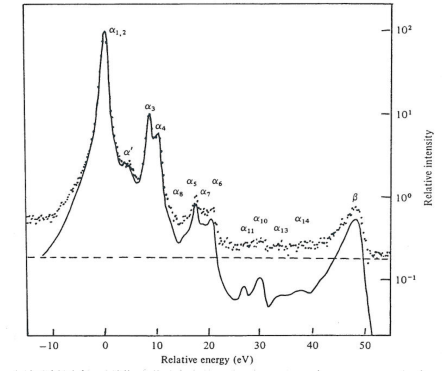
\includegraphics[scale=4.5]{figures/04_06.png}
	\caption{The relative intensity of X-rays emitted from a magnesium anode plotted relative to the $K_{\alpha 12}$ energy. Notice that the intensity is on a logarithmic scale \cite{krause}.}
	\label{fig:mganode}
	\end{center}
\end{figure}

Shown in Table \ref{tab:satlines} are the X-ray satellite lines of magnesium and aluminium positioned relative to the main lines. Notice that more than \SIrange{10}{15}{\percent} of the X-ray intensity will be in the different satellite structures. All these various problems with different X-ray lines can be avoided if we let the X-ray pass a monochromator. This is easily established by diffraction of the X-rays in a Si single crystal. The only major drawback using this procedure is the extensive loss of sensitivity (actually photon intensity) and naturally the investments. Therefore another approach is used when high resolution is called for.

\begin{table}
\begin{center}
\caption{Relative intensity and shift of various satellite lines compared to the main line.}\label{tab:satlines}
\begin{tabular} {|l|r|r|} \hline
          X-ray Line & Shift [\si{\electronvolt}] & Relative Intensity [\si{\percent}]\\ \hline
          Mg$_{K_{\alpha 12}}$ & 0.0 & 100 \\ \hline Mg$_{K_{\alpha
          '}}$ & 4.5 & 1.0 \\ \hline Mg$_{K_{\alpha 3}}$ & 8.4 & 9.2 \\
          \hline Mg$_{K_{\alpha 4}}$ & 10.0 & 5.1 \\ \hline
          Mg$_{K_{\alpha 5}}$ & 17.3 & 0.8 \\ \hline Mg$_{K_{\alpha
          6}}$ & 20.5 & 0.05 \\ \hline Mg$_{K_{\beta}}$ & 48.0 & 2.0
          \\ \hline
          Al$_{K_{\alpha 12}}$ & 0.0 & 100  \\ \hline Al$_{K_{\alpha '}}$ &
          5.6 & 1.0  \\ \hline Al$_{K_{\alpha 3}}$ & 9.6 & 7.8  \\
          \hline Al$_{K_{\alpha 4}}$ & 11.5 & 3.3  \\ \hline
          Al$_{K_{\alpha 5}}$ & 19.8 & 0.4  \\ \hline Al$_{K_{\alpha
          6}}$ & 23.4 & 0.3  \\ \hline Al$_{K_{\beta}}$ & 70.0 & 2.0  \\
          \hline
\end{tabular}
\end{center}
\end{table}

By using synchrotron facilities it is possible to obtain an extremely brilliant source of X-rays in a broad spectrum of energies (\SIrange{10}{1000}{\electronvolt}). The radiation is formed by confining high energy electrons (\SI{5}{G\electronvolt}) into a storage ring, a so-called synchrotron. Accelerated electrons will emit radiation. By establishing suitable  monochromators it is possible to select the desired photon energy. This has many advantages experimentally since the photon energy is tuneable (meaning it is possible to select a photon energy where maximum surface sensitivity is obtained)  and the broadening can be controlled. The  only major drawback on this type of equipment is that it is huge and  expensive facilities, located only a few places in Europe.

\section{Spectral Interpretation}
Now all the equipment has been established for doing the XPS experiment. A typical XPS spectrum of Cu(100) is shown in \autoref{fig:cuxps} where the source is the Al$_{K_{\alpha 4}}$ radiation from a conventional dual Al/Mg X-ray source. The observed spectrum is a mapping of the energy levels in copper. The features at the highest kinetic energy, i.e. zero binding energy, are from the valence region of copper. This is not very intensive and can hardly be seen.

\begin{figure}[h!]
	\begin{center}
	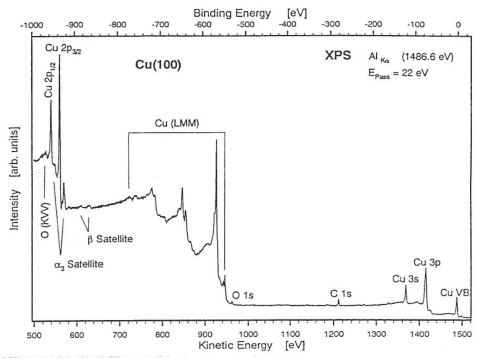
\includegraphics[width=\textwidth]{figures/04_07.png}
	\caption{XPS spectrum of a Cu(100) surface measured using a HSA analyser.}
	\label{fig:cuxps}
	\end{center}
\end{figure}

The small feature that is seen here is the 3d level lying just below the Fermi level. Proceeding towards higher binding energies the 3p and 3s levels around \SI{65}{\electronvolt} and \SI{110}{\electronvolt} respectively. The Auger  lines follow naturally from the relaxation of the  holes  that  has  been created by the photoemission process. They are not very interesting in this context and we shall leave the discussion of these to the next chapter. At even higher binding energies we find first  the 2p$_{\frac{3}{2}}$ and then the 2p$_{\frac{1}{2}}$ lines. Contrary to the  3p line the spin orbit splitting is very obvious and amounts to roughly \SI{20}{\electronvolt}. This splitting will be present for all subshells with an angular momentum higher than zero. Thus the only lines where no splitting should be expected are the lines due to excitations of s electrons. For careful studies of the surfaces it may be informative to take a closer look at the high energy region of the spectrum as shown in \autoref{fig:cuxpszoom}. It is now easily seen that this surface is contaminated as all the lines cannot be accounted for by copper. Carbon, oxygen and sulphur are easily identified in non-vanishing amounts. Furthermore, it is also possible to identify ghost-peaks from the Mg$_{K\alpha}$ anode, which are excited when the aluminium source is used. Even some $\beta$ satellites from the Cu$_{2p}$ lines can be observed. All such features has to be accounted for in a detailed XPS study.

\begin{figure}[h!]
	\begin{center}
	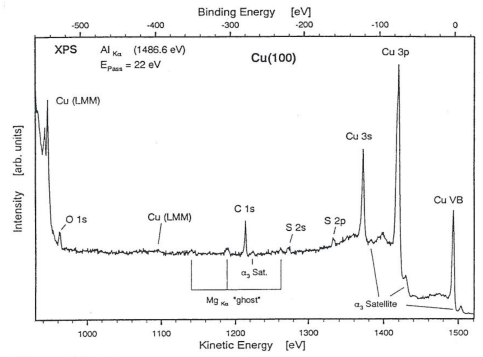
\includegraphics[width=\textwidth]{figures/04_08.png}
	\caption{As \autoref{fig:cuxps} but rescaled and only showing the region above \SI{965}{\electronvolt} kinetic energy.}
	\label{fig:cuxpszoom}
	\end{center}
\end{figure}

\subsection{Multiplet splitting in XPS}
To understand the various features observed by XPS we must look a little into atomic physics. In the following we shall treat all atoms as if they initially have filled shells, i.e. we will disregard the valence electrons which are highly delocalised in metals. All the electron energy levels can now be determined by finding a solution to the Schr\"{o}dinger equation with the appropriate Hamiltonian. This can be done iteratively by a self consistent Hartree-Fock calculation. In this case all electron energy levels like 1s, 2s, 2p, 3p, and 3d for the copper atom will be degenerate. This state will in the following be referred to as the {\em initial state}. This degeneracy of a level will be lifted if an electron is being excited out of the atom leaving a hole in a subshell, say, 2p. The same calculation has to be performed for this system, now referred to as the {\em final state}, but now the spin-orbit interaction also has to be taken into account since we have an unpaired hole \footnote{A missing electron in an otherwise full shell is equivalent to having only one electron in an otherwise empty shell, except that the spin-orbit interaction changes sign.}. The spin-orbit coupling is treated as a perturbation of the system and in the present case it is convenient to formulate a new quantum number $j$ instead of the angular momentum $l$ and the spin $s$ as $\vec{j}=\vec{l}+\vec{s}$. As $\vec{s}$ only can take the values $+\frac{1}{2}$ and $-\frac{1}{2}$ and as $j$ only can take the values

\begin{equation}
l+s \geq j \geq \mid l-s \mid
\end{equation}

\noindent it is obvious why there will always be a splitting for levels with $l\neq 0$. The intensity distribution in the two lines will be given by the degeneracy in the two final states which is $2j+1$.  Thus  the intensity ratio between the two 2p lines observed in \autoref{fig:cuxps} is 4:2. The same formalism can be used to understand the splitting observed in the 2p, 3d, and  4f shells shown in \autoref{fig:xpssplitting} \cite{siegbahn1}.

\begin{figure}[h!]
	\begin{center}
	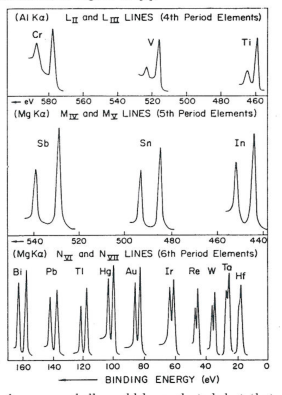
\includegraphics[scale=4.5]{figures/04_09.png}
	\caption{The XPS spectra of a variety of elements showing the development in spin-orbit splitting for the 2p, 3d and 4f levels.}
	\label{fig:xpssplitting}
	\end{center}
\end{figure}

This was for the simple case where open shells could be neglected, but that is not always the case. If we consider the rare earth metals (which by no means are rare) the 4f shell will be very localised on the atom although it is weakly bound. This is due to the lanthanide contraction and the same phenomenon applies to the actinides. Thus when going through the lanthanide's series where the 4f shell is being filled, the chemistry is not changing because the outermost electron configuration is basically not changing. This also has a strong influence on the observed XPS spectra of these metals. \autoref{fig:ybxps} shows one of the relatively  simple examples of multiplet splitting \cite{chorkendorff}.

\begin{figure}[h!]
	\begin{center}
	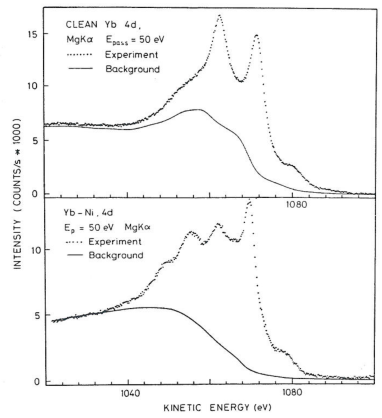
\includegraphics[scale=4.5]{figures/04_10.png}
	\caption{XPS spectrum of a) pure Ytterbium and b) an Ytterbium-Nickel alloy. The fully drawn line represents the background due to inelastic energy losses during the transport.}
	\label{fig:ybxps}
	\end{center}
\end{figure}

In the top panel of \autoref{fig:ybxps} the 4d region of pure ytterbium is shown. As it  has the electron configuration [Xe]4f$^{14}$6s$^{2}$ it is a divalent metal with  otherwise filled shells. Thus the 4d region should just show a simple 4d$_{\frac{5}{2}}$ and 4d$_{\frac{3}{2}}$  splitting. At first glance it looks like it does not have the correct intensity distribution, but this can easily be explained by the background of electrons that has undergone energy losses from deeper layers. The background can be estimated as a solid line as shown in \autoref{fig:ybxps} by studying the energy loss spectra of pure Yb. In order to get a clear view of the feature it has been subtracted and the "true" spectrum  is shown in \autoref{fig:ybxpsnobackground} together with a fit taking into account the appropriate X-ray satellites \cite{chorkendorff}.

\begin{figure}[h!]
	\begin{center}
	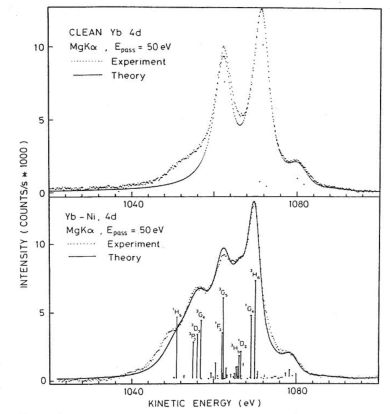
\includegraphics[scale=4]{figures/04_11.png}
	\caption{The background corrected spectra of \autoref{fig:ybxps} shown together with theoretical fits relying on multiplet splitting.}
	\label{fig:ybxpsnobackground}
	\end{center}
\end{figure}

The fit is quite reasonable although not perfect. The reason for the discrepancy is that intrinsic energy loss mechanisms are not included in the background subtraction which is only dealing with the transport of electrons out of the material.

Now if ytterbium is evaporated onto nickel and the sample is heated slightly an alloy is formed and the Yb 4d region changes completely as shown in the lower panel of \autoref{fig:ybxps} and \autoref{fig:ybxpsnobackground}. This change can be understood in terms of a change of valence of Yb from being divalent to becoming trivalent. A trivalent Yb atom will initially have a hole in the 4f shell so the final state after the photoemission process will be an atom with a hole both in the 4f shell and one in the 4d shell. These two holes will interact strongly through electrostatic interaction. This sort of interaction is treated well through the so-called Russell-Saunders coupling scheme or LS-couplings scheme where the two angular moments $l_1$ and $l_2$ are coupled to L and similar for the two spin values. This immediately leads to large numbers of different final states, $L=1,2,3,4,5$ and $S=0,1$, which usually are described through the terms

\vspace{0.3cm}

\noindent $^{1}P, ^{3}P, ^{1}D, ^{3}D, ^{1}F, ^{3}F, ^{1}G, ^{3}G, ^{1}H, ^{3}H$

\vspace{0.3cm}

\noindent a number of singlet or triplet states ($^{(2S+1)}X$). All these ten terms have different energies and will therefore appear in the spectrum. However, this is not all. We have not considered the spin orbit coupling. When that is taken into account $l$ and $s$ are no longer good quantum numbers. By treating the spin-orbit coupling as a perturbation a new set of eigenvalues can be developed on the basis set of $L$ and $S$ states and the new coupling scheme will be the so- called intermediate coupling scheme where $\vec{J} = \vec{L}+\vec{S}$ are the good quantum numbers. The result of this extra perturbation is that the degeneracy of the triplet states is lifted and each of these splits up in three different states. There will now be 20 final states

\vspace{0.3cm}

\noindent $^{1}P_{1}, ^{3}P_{0}, ^{3}P_{1}, ^{3}P_{2}, ^{1}D_{2}, ^{3}D_{1}, ^{3}D_{2}, ^{3}D_{3}, ^{1}F_{3}, ^{3}F_{2}, ^{3}F_{3}, ^{3}F_{4}, ^{1}G_{4}, ^{3}G_{3}, ^{3}G_{4}, ^{3}G_{5},\\
^{1}H_{5}, ^{3}H_{4}, ^{3}H_{5}, ^{3}H_{6}$
          
\vspace{0.3cm}

The intensities for the various final states are not given by a simple expression due to the mixing of various $LS$ states. All these and the appropriate $\alpha_{34}$ X-ray satellites are taken into account in \autoref{fig:ybxpsnobackground} and a good fit is obtained. Thus XPS is very useful for determination of the electronic configuration in such cases.

\autoref{fig:ybvalence} shows the valence band region of Yb studied with a synchrotron facility where the photon frequency is tuneable \cite{gerken}. The valence  electrons  (6s6p)$^{2}$ can just be observed for the lowest photon energies as a step function at the Fermi level. In this region we should expect a simple doublet resulting from the filled 4f shell, however two doublets are observed.

\begin{figure}[h!]
	\begin{center}
	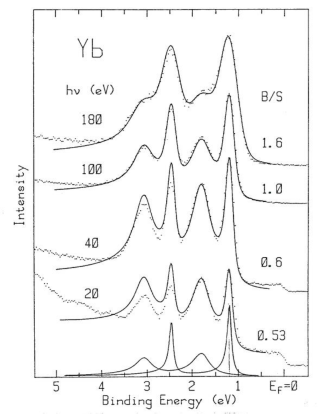
\includegraphics[scale=4]{figures/04_12.png}
	\caption{The valence band region of ytterbium excited by synchrotron light with increasing energy \cite{gerken}.}
	\label{fig:ybvalence}
	\end{center}
\end{figure}

By increasing the photon energy it is clearly seen that the doublet at the higher binding energy disappears. If we choose to look at the same region with XPS we actually only observe a single doublet. This shows how the surface sensitivity changes with energy (see Fig. \ref{fig:ybvalencecomp}) \cite{gerken}. The electrons are in this case essentially emitted with the photon energy and we should therefore expect low surface sensitivity when the photon energy is high. Thus the doublet observed at high energy is due to signal from the bulk of the material, whereas the extra doublet observed at low photon energy is due to the surface region. As we shall see, the bonding energy of the electron is dependent not only on the atom and its electron configuration,  but  also  on  the chemical surroundings of the atom. In this case the surface atoms are missing a number of neighbours compared to those sitting in the bulk. They will therefore be located in a different electron density which will change the energy of the emitted electron  from the bulk value. The observed spectra shown in \autoref{fig:ybvalence} allows for an estimation of the inelastic mean free path which in the present case was found to be roughly \SI{4}{\angstrom} at \SI{20}{\electronvolt} and \SI{10}{\angstrom} at \SI{180}{\electronvolt}.

\begin{figure}[h!]
	\begin{center}
	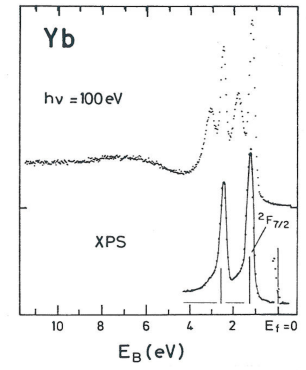
\includegraphics[scale=3.5]{figures/04_13.png}
	\caption{Comparison between the valence band region of ytterbium excited by \SI{100}{\electronvolt} photons and by Al$_{K\alpha}$ radiation \cite{gerken}.}
	\label{fig:ybvalencecomp}
	\end{center}
\end{figure}

The alloying and change in electron configuration of the Yb could just as well have been studied by following the region of the 4f electrons. This demonstrates how surface reactions between metals can be followed quite nicely especially if monochromatised synchrotron light is used.

\subsection{The Binding Energy in XPS}
Since the binding energy of the various shells is characteristic for each element, as can be seen from \autoref{fig:bindingenergies}, this in itself allows for identification of the elements. In the previous section we assumed that the kinetic energy of the emitted electron was given by

\begin{equation}
E_{kin}=h\nu-E_B-\Phi
\end{equation}

\begin{figure}[h!]
	\begin{center}
	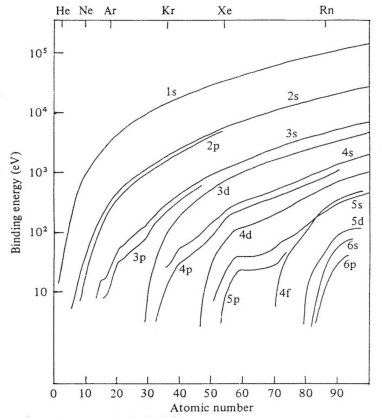
\includegraphics[scale=4]{figures/04_14.png}
	\caption{The binding energy for a broad variety of levels as a function of atomic number \cite{siegbahn1}.}
	\label{fig:bindingenergies}
	\end{center}
\end{figure}

In the following we will disregard $\Phi$ and concentrate on the binding energy $E_{B}$. It was earlier assumed that the electron configuration of the atom (except for some splitting) did not change by the photoemission i.e. the energy of all other electrons is the same as before the photoemission process. This energy is referred to as the Koopman's energy. However, this is never observed  because the atom is a dynamical system which immediately relaxes during the  process screening out the hole made in the core level. Thus higher lying electrons will in principle feel the core change from $Z$ to approximately $Z+1$ whereby they will obtain a higher binding energy. The relaxation will result in a photoelectron with a higher kinetic  energy. The gain in energy we shall call the  atomic  relaxation, $E_{ar}$. Including this term the kinetic energy for an atom will be

\begin{equation}
E_{kin}=h\nu-E_{B}+E_{ar}
\end{equation}

This is only true if the photoemission process is an adiabatic process, i.e. the emission process is slow enough for equilibrium to be obtained. This is not true for the photoemission process where the sudden approximation scheme is much more applicable. All electrons will feel a sudden change in potential which may sometimes lead to excitations of other electrons in the atom. As the ionised atom may now be left in an excited state there will be less energy for the emitted photoelectron and a lower kinetic energy will be measured. The result will therefore be that a number of satellites which will be observed towards lower kinetic energy. An example of such a phenomenon is shown in \autoref{fig:xe3d} where the Xe 3d spectrum is shown.

\begin{figure}[h!]
	\begin{center}
	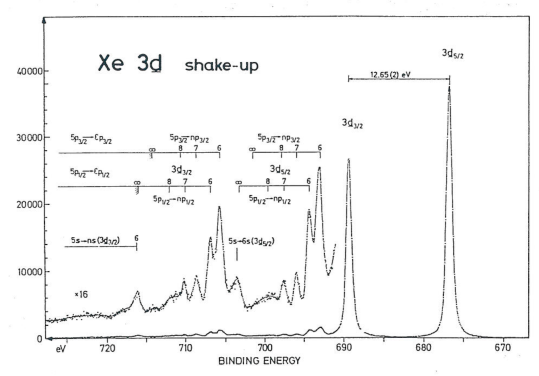
\includegraphics[width=\textwidth]{figures/04_15.png}
	\caption{The 3d region of atomic Xe clearly showing shake up-satellites \cite{siegbahn1}.}
	\label{fig:xe3d}
	\end{center}
\end{figure}

The two parent lines are easily identified, but notice the rich structure towards the higher binding energy, which is mainly due to a simultaneous excitation of the 5p electrons to various empty levels. This process is called a shake-up process as the electrons are excited to bound states. If they are excited to the continuum they are called shake-off satellites. The real origin of this phenomenon we shall find in the many-body description of the atom. In an accurate description of an atom it is  usually necessary to invoke Configuration Interaction (CI). Neither the initial state ($\Psi_{i}$) nor the final state  $\Psi_{f}$ can be described by a single  electron configuration but are described by a linear combination of wave-functions  for different configurations with different energies. Thus when forming  the matrix element for finding the  transition probability there will be possibilities for some atoms to have strong components of various electron configurations as seen in \autoref{fig:xe3d}.  In most cases only configuration interaction has to be considered for the  final state. For further details on this effect the reader is referred to \cite{shirley}.

Let us now consider an atom embedded in a metal. Naturally we will still have the atomic relaxation but now another effect will also influence the kinetic energy of the photoelectron. The weakly bound and delocalised valence electrons will be able to respond swiftly to the potential changes set up by the photoemission process. Charge will flow in and screen the emitted electron from the ionised atom resulting in a higher kinetic energy (see Fig. \ref{fig:atomicrelax}).

\begin{figure}[h!]
	\begin{center}
	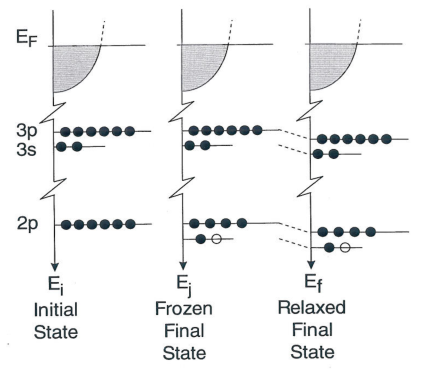
\includegraphics[scale=3]{figures/04_16.png}
	\caption{Sketch showing the effect of extra atomic relaxation in a metal.}
	\label{fig:atomicrelax}
	\end{center}
\end{figure}

This contribution shall be called extra atomic relaxation $E_{ear}$ which results in the kinetic energy

\begin{equation}
E_{kin}=h\nu-E_{B}+E_{ar} +E_{ear}
\end{equation}

The size of $E_{ar}$ and $E_{ear}$ can be up to \SIrange{10}{15}{\electronvolt} so a substantial difference between the spectra of an element in the vapour phase and in the solid state can be observed (see Fig. \ref{fig:atomicrelax}). Just as in the atomic case the sudden approximation may lead to excitation of various states. As we are considering a solid there will be no discrete levels above the Fermi level but a band structure so that the CI-picture is not appropriate. Instead we can just consider some of the energy loss mechanisms we discussed in Chapter \ref{ch:reqs}. Excitations of excitons is equivalent to the shake-up satellites and also excitations of plasmons may be observed. These intrinsic energy losses have to be distinguished from those observed in conjunction with the transport of the electrons through the solid which we shall call extrinsic energy losses. In \autoref{fig:ybxps} we subtracted a background due to the transport of the electrons through the Yb.  However, some discrepancy is still observed in the background corrected spectra when fitted  with a theoretical line shape. The observed discrepancy can be explained by a so-called intrinsic energy loss to a plasmon created by the sudden potential change during the photo emission process. The effect of intrinsic excitons are naturally very difficult to separate experimentally from the extrinsic, but they  can easily be observed in for instance the Pt 4f spectrum shown in \autoref{fig:pt4f} \cite{wertheim}.

\begin{figure}[h!]
	\begin{center}
	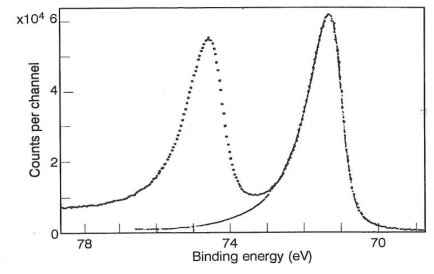
\includegraphics[scale=3.5]{figures/04_17.png}
	\caption{The 4f region of platinum displaying an asymmetrical peak shape.}
	\label{fig:pt4f}
	\end{center}
\end{figure}

A priori a Lorentzian line shape is to be expected as the broadening primarily is determined by the lifetime of the final state. It is, however, clearly seen that the two lines are slightly asymmetrical towards lower kinetic energy. Usually this sort of line can be fitted by a Doniach-Sunjic line shape which is asymmetrical \cite{doniach} and explained by excitations of excitons.

The separation of the lines in their different components is very important for obtaining a high accuracy on quantitative determinations of surface compositions. It is therefore very important to understand the origin of the various effects.

So far  we have only discussed the influence of the final state on the binding energy. Different chemical surroundings will also affect the initial state as the electron configuration and density around the atom will be changed. This change in binding energy related to various chemical surroundings is called the chemical shift. However, the final state will also be sensitive to the chemical state of the atom. Thus the phenomenon can only be separated in an initial and a final state effect from a theoretical point of view. The kinetic energy can formally be written as

\begin{equation}
E_{kin}=h\nu-E_{B}+E_{ar}+E_{ear}+E_{chem}
\end{equation}

\noindent where $E_{chem}$ is dependent on the surroundings of the atom.

An example of a chemical shift is illustrated in \autoref{fig:tiox} where the 2p region of Ti and \ce{TiO2} are depicted \cite{perkin}.

It is clearly seen that the Ti 2p lines are shifts roughly \SI{4.5}{\electronvolt} towards higher binding energy by oxidation into \ce{TiO2}. This sort of data has been measured for a number of chemical compounds and the results are shown in \autoref{fig:ti2p} for Ti \cite{perkin}.

Notice how the binding energy increases with increasing electronegative neighbours. Such information  only gives an indication of the chemical state of a surface, but in combination with the possibility to identify which elements are present else and how much, this can be  valuable information. One area where the chemical shift plays a strong role is within the field of polymer research where it can be used to identify the role of functional groups and their behaviour by adhesion. As an example the XPS spectrum of ethyltrifluroacetate (\ce{C4H5F3O2}) is shown in \autoref{fig:cshift} where four lines of carbon are easily  identified \cite{ghosh}.

Sometimes the chemical shift will also be followed by a change in the availability to excite different satellites. This is clearly seen from \autoref{fig:cushift} where the copper 2p region undergoes a chemical shift of roughly \SI{1}{\electronvolt} by oxidation, but at the same time a strong feature with equal intensity to the main line is observed at \SI{10}{\electronvolt} higher binding energy \cite{perkin}.

\begin{figure}[h!]
	\begin{center}
	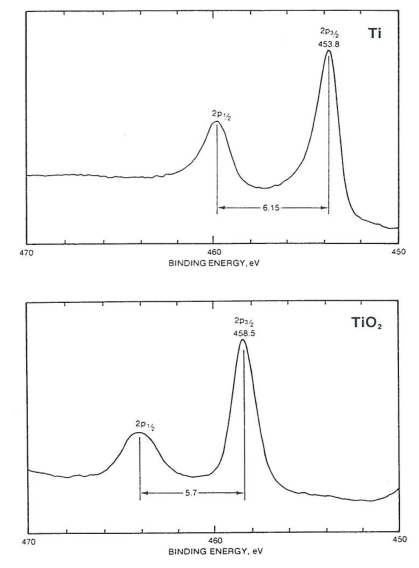
\includegraphics[scale=4]{figures/04_18.png}
	\caption{The chemical shift of Ti upon oxidation \cite{perkin}}
	\label{fig:tiox}
	\end{center}
\end{figure}

\begin{figure}[h!]
	\begin{center}
	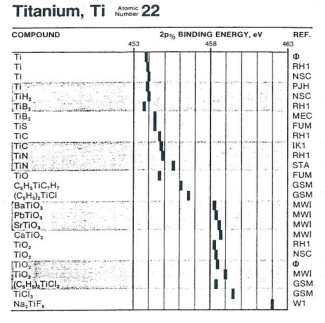
\includegraphics[scale=4]{figures/04_19.png}
	\caption{The Ti 2p line position for various chemical compounds \cite{perkin}.}
	\label{fig:ti2p}
	\end{center}
\end{figure}

\begin{figure}[h!]
	\begin{center}
	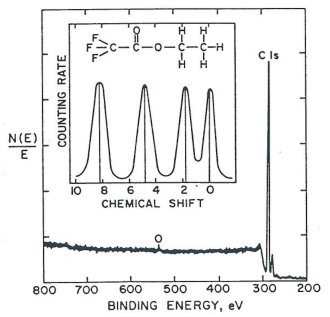
\includegraphics[scale=4]{figures/04_20.png}
	\caption{The chemical shifts of carbon in ethyltrifluroacetate.}
	\label{fig:cshift}
	\end{center}
\end{figure}

\begin{figure}[h!]
	\begin{center}
	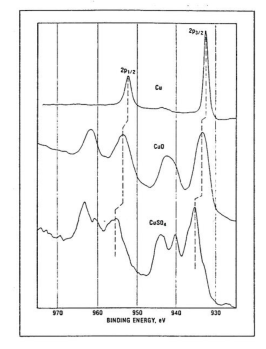
\includegraphics[scale=5]{figures/04_21.png}
	\caption{The chemical shift of copper and the satellite structure \cite{perkin}.}
	\label{fig:cushift}
	\end{center}
\end{figure}

\subsection{Line Width}
Especially when chemical shifts and  electron structures are studied it is important to consider the line width of the XPS lines. Ideally both the energy  distribution of the X-ray line and the  energy distribution of an emitted electron should be given by the lifetime of the holes left behind (if we disregard any contribution from intrinsic and extrinsic energy losses) and the line shape should therefore be described by a Lorentzian which has the form

\begin{equation}
L(E)= \frac{A}{(E-E_0)^2+\frac{\Gamma^2}{4}}
\end{equation}

\noindent where $\Gamma$ corresponds to the FWHM. If there were no other sources of  broadening the lines than these two, the
resulting XPS line shape would be given by

\begin{equation}
P(E)=L_{X-ray}(E)*L_{Photoemission}(E)
\end{equation}
          
\noindent where * refers to a convolution of the two line shapes. The analyser will, however, also always contribute to the broadening of the observed lines. This broadening can usually be described adequately by a Gaussian line shape

\begin{equation}
G(E)=Be^{-\frac{4ln(2)(E-E_0)^2}{\Gamma^2}}
\end{equation}

\noindent where $\Gamma$ again corresponds to the FWHM. Thus in order to find the resulting line shape the line shape $P(E)$ also has  to be convoluted by $G(E)$

\begin{equation}
R(E)=P(E)*G(E)
\end{equation}

The resulting line shape $R(E)$ can be approximated by a Gaussian and the resulting FWHM can be approximated by

\begin{equation}
\Gamma_{res}=\sqrt{\Gamma_{X-ray}^2+\Gamma_{Photoemission}^2+\Gamma_{Analyser}^2}
\end{equation}

If for example $\Gamma_{X-ray}=\SI{0.85}{\electronvolt}$ and $\Gamma_{Photoemission}^{2}=\SI{0.5}{\electronvolt}$ it would then not be meaningful to press the resolution of the  analyser much below \SI{0.5}{\electronvolt} since this would just lead to loss of signal without any significant gain in resolution. As the signal to noise ratio ideally will be proportional to $\sqrt{Intensity}$ it is important always to counter-balance resolution and intensity.

\subsection{The Transition Probability}
The probability for excitation of an electron from an atom when interacting with an X-ray photon can be described in quantum mechanics as an interaction between the initial and final state through an interaction Hamiltonian. This Hamiltonian can be approximated by the time-dependent electric field and the problem can be solved by use of time-dependent perturbation theory leading to Fermi's Golden rule:

\begin{equation}
P\propto |<\Phi_{initial}|H_{int}(t)|\Phi_{final}>|^2
\end{equation}

By such a calculation it is possible to estimate the cross section per X-ray photon to excite a photoelectron. The cross section is dependent on the photon  energy and is, as can be seen from \autoref{fig:csan} also very dependent on which shell is considered. The above calculation relies on the assumption that the initial and final states can be described by one electron wave functions, though it should not be expected to be very accurate. It will for example not be able to describe many-body effects like the shake-up and shake-off satellites, but it gives a good indication of which photoemission lines are accessible.

\begin{figure}[h!]
	\begin{center}
	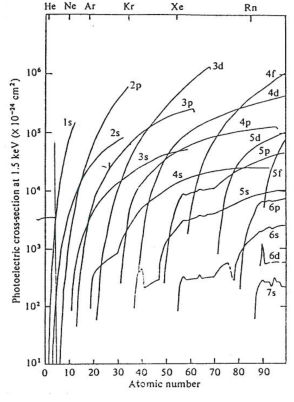
\includegraphics[scale=4]{figures/04_22.png}
	\caption{The calculated cross-sections for \SI{1.5}{k\electronvolt} photons for various levels as a function of atomic number \cite{shofield}.}
	\label{fig:csan}
	\end{center}
\end{figure}
             
It is obvious, from \autoref{fig:csan}, that it
will be very difficult (= impossible) to measure the photoemission lines of hydrogen and helium by Al$_{K\alpha}$ radiation. Concerning the satellites, there exists a sum rule saying that the cross section determined by the above one electron approximation equals the cross section for all the possible satellites and the parent line in the many body picture. Thus if strong satellites are involved, like seen in the copper oxide, special care should be taken using these calculated cross sections. Due to the various uncertainties of the calculated cross section, it is much more common but not without problems to rely on empirical parameters for quantitative analysis by XPS.

\section{Quantitative XPS Analysis}
When a surface is exposed to X-rays there  will be the following probability for emission of a photoelectron per incident photon

\begin{equation}
P_{xk}=\sigma_{xk}N_xt
\end{equation}

\noindent where $\sigma_{xk}$ is the cross section of level $k$ in the element $x$, $N_x$ is the concentration (\si{atoms\per cm^3})  of element $x$ in the surface, and $t$ is  the thickness of the probed area. The probability for exciting electrons in the sample is not the interesting number, what is interesting is the probability for those electrons to escape the surface without undergoing energy losses. If we assume that the surface is homogeneous ($N_{x}(z) = N_{x} for t\gg \lambda_{xk}$) the probability for getting the electrons outside the sample, emitted from a depth of $z$, can be approximated by

\begin{equation}
dP_{xk}\prime(z)=\sigma_{xk}N_xe^{-\dfrac{z}{\lambda_{xk}}}dz
\end{equation}

\noindent which by integration over all depths leads to

\begin{eqnarray}
P_{xk}\prime	& =	& \sigma_{xk}N_x\int_0^{\infty}
          e^{-\dfrac{z}{\lambda_{xk}}}dz\\
P_{xk}\prime	& =	& \sigma_{xk}N_x\lambda_{xk}
\end{eqnarray}

Here $\lambda_{xk}$ is the inelastic mean free path for an electron emitted from level $k$ travelling through material $x$. Thus the probability of emitting electrons beyond an infinitely thick sample will always be the same as if we were looking at a sample of thickness $\lambda_{xk}$ without any damping. The X-ray will always penetrate deeply into the surface and excite atoms, but the rather small mean free path for the photoelectrons ensures the surface sensitivity as indicated in \autoref{fig:pendepth}.

The number of electrons detected from  shell $k$ of element $x$ will, besides the above probability, be proportional to  the number of photons $F_{h\nu}$ and the  transmission function for the analyser used $T(E_{kx}$)

\begin{equation}
I_{xk}=\sigma_{xk}N_x\lambda_{xk}F_{h\nu}T(E_{xk})
\end{equation}

This is the important formula for determining the composition of a surface which is homogeneous.\\

The intensity contribution from a layer in the depth $z$ of thickness $dz$ will be

\begin{eqnarray}
dI_{xk}	& =	& dP_{xk}\prime(z)F_{h\nu}T(E_{xk})\\
	& =	& \sigma_{xk}N_xe^{-\dfrac{z}{\lambda_{xk}}}F_{h\nu}T(E_{xk})dz\\
	& =	& \frac{I_{xk}}{\lambda_{xk}}e^{-\dfrac{z}{\lambda_{xk}}}dz \label{eq:intcontr}
\end{eqnarray}

\subsection{Example}
Estimate the surface composition of an alloy made of \ce{NiSi} assuming it to be homogeneous. The Intensity ratio $I_{\mathrm{Si}2p}/I_{\mathrm{Ni}3p}$ is found to be 0.20. The cross section for the two lines can be found in \autoref{fig:csan} to be \SIlist{1e-20;2.5e-20}{cm^{-2}} for Si and Ni respectively. Since the binding energy for the two lines is nearly the same (see Fig. \ref{fig:bindingenergies}) it is safe to assume that

\begin{equation}
\frac{I_{\mathrm{Si}2p}}{I_{\mathrm{Ni}3p}}=\frac{\sigma_{\mathrm{Si}2p}N_{\mathrm{Si}}\lambda_{\mathrm{Si}2p}F_{h\nu}T(E_{\mathrm{Si}2p})}{\sigma_{\mathrm{Ni}3p}N_{\mathrm{Ni}}\lambda_{\mathrm{Ni}3p}F_{h\nu}T(E_{\mathrm{Ni}3p})}
\end{equation}

\noindent can be approximated by

\begin{equation}
\frac{I_{\mathrm{Si}2p}}{I_{\mathrm{Ni}3p}}=\frac{\sigma_{\mathrm{Si}2p}N_{\mathrm{
Si}}}{\sigma_{\mathrm{Ni}3p}N_{\mathrm{Ni}}}
\end{equation}

whereby the atomic composition can be estimated suggesting a \ce{Ni2Si} alloy.

\begin{figure}[h!]
	\begin{center}
	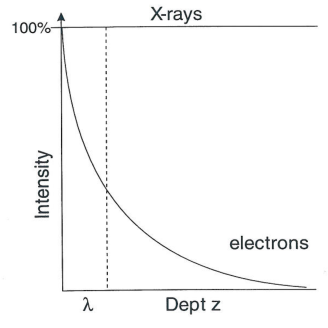
\includegraphics[scale=3]{figures/04_23.png}
	\caption{Sketch showing the difference in penetration depth of electrons and X-rays.}
	\label{fig:pendepth}
	\end{center}
\end{figure}

The mean free path can alternatively be estimated from \autoref{fig:mean_free_path} and the transmission function can be determined so this method can be used more generally. However, these different parameters are often put together in what is called a sensitivity factor $S_{xk}$ which then is determined for a certain type of analyser. The intensity of a line can then be determined as the area of the XPS line (or less accurate simply the peak height) and would then be given by

\begin{equation}
I_{xk}=S_{xk}N_xF_{h\nu}
\end{equation}

and the atomic concentration of each element present in the sample can then be estimated as

\begin{equation}
C_{x}=\frac{\frac{I_{xk}}{S_x}\times\SI{100}{\percent}}{\sum_{i=1}^N\frac{I_i}{S_i}}
\end{equation}

where $i$ refers to only one subshell in any of the $N$ observed elements. Also in this case it is assumed that the surface is homogeneous. More elaborate estimations can be done without this assumption, but they will always be model dependent.

The surface sensitivity can be improved considerably if the surface of the  sample is tilted relative to the analyser as shown in \autoref{fig:angle}.

\begin{figure}[h!]
	\begin{center}
	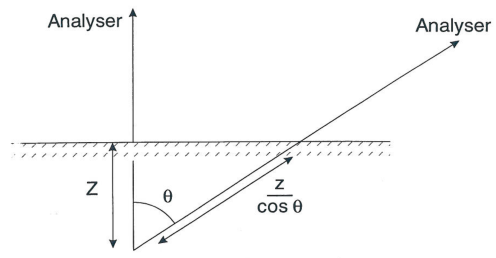
\includegraphics[scale=3]{figures/04_24.png}
	\caption{Sketch showing the effect of a take-off angle $\theta$.}
	\label{fig:angle}
	\end{center}
\end{figure}

In this manner the electrons emitted from the depth $z$ will now have to pass through a layer of thickness $z/cos(\theta)$ where $\theta$ is the angle between the surface normal and the analyser. If we consider a thin overlayer of material $y$ of thickness $d$ on top of layer $x$ we will by integration of Eq. \eqref{eq:intcontr} get 

\begin{equation}\label{eq:intang}
I_{xk}(d)=I_{xk}e^{-\dfrac{d}{cos(\theta)\lambda_{yk}}}
\end{equation}

\noindent and

\begin{equation}
I_{yk\prime}(d)=I_{yk\prime}\left(1-e^{-\dfrac{d}{cos(\theta)\lambda_{yk\prime}}}\right)
\end{equation}

Thus by varying the angle it is possible to determine if the surface is inhomogeneous in the outermost layers or if it has another electron structure as we saw it in the ytterbium case. Naturally surfaces are not homogeneous, there are several reason why this is not the case. For example the spectra of the Cu(100) single crystal shown in Figures \ref{fig:cuxps} and \ref{fig:cuxpszoom} clearly show traces of contaminations that will be confined to the surface. The oxygen and carbon are due to contamination since the crystal has been standing in the vacuum chamber for an extended period without cleaning. The presence of the sulphur, however, is due to segregation from the bulk of the crystal, which under the heat treatment necessary to anneal the crystal and re-establish the order after the cleaning procedure (argon sputtering) has diffused out at the surface. The amount of sulphur in the crystal amounts to the ppm level, but as the sulphur has a much lower surface energy than copper it is energetically favourable for the system to have the sulphur on the surface. This is a quite general phenomenon and most alloys will therefore be enriched in one component at the surface compared to the bulk values.

The above formalism can be refined in  several ways (see \cite{briggs} and the references  therein). We shall not deal further with these problems here, but just mention that one of the major problems when performing quantitative analysis by XPS is the subtraction of the background in the spectra. The intensity mentioned above is proportional to the area of the XPS line, thus the underlying background  due  to  electrons that have undergone energy losses should be eliminated just as it was done in \autoref{fig:cuxps}. In general the energy loss function is not known well enough that such a procedure can be used, and even when it was we saw that there was still a discrepancy because of the intrinsic energy losses. Thus quantitative analysis with XPS will always have a rather large uncertainty and results better than \SI{10}{\percent} should never be expected. The satellites will always be a source of errors and the assumption of a homogeneous sample is usually only fulfilled for pure elements. Nevertheless, XPS has proven extremely useful in many cases and no other method for determining the surface composition  as accurately as XPS exists today.

\newpage
\section{Problems}
\begin{enumerate}
\item What is the fundamental reason for the surface sensitivity of the electron spectroscopic methods?

\item Are there elements which cannot be detected by XPS? What about AES?

\item We want to determine the mean free path of electrons in iron by using the method described in the notes. Thus iron is deposited on a substrate of Ni and the damping of the Ni lines are measured. Two photoemission lines from Ni are used (excitation by Al$_{k\alpha}$) which are observed at \SIlist{65;700}{\electronvolt} binding energy, respectively. Due to the geometry of the experimental set-up only electrons in an angle of \ang{60} from the surface normal will be detected. The intensity of the XPS signal before any deposition was measured to be $I_{\SI{65}{\electronvolt}}=\SI{10000}{counts\per s}$ and $I_{\SI{700}{\electronvolt}}=\SI{60000}{counts\per s}$. Now \SI{8.6e-7}{g\per cm^2} of iron is deposited whereby the two lines are reduced to $I_{\SI{65}{\electronvolt}}=\SI{2300}{counts\per s}$ and $I_{\SI{700}{\electronvolt}}=\SI{6600}{counts\per s}$. Under which assumption can we estimate the mean free path of the electrons in iron? Make the assumption and estimate the mean free paths.

Suggest/discuss a method to estimate when \SI{8.6e-7}{g\per cm^2}of iron has been deposited.

\item XPS is used to check whether a Ni(100) single crystal is clean enough to be used for surface reactivity experiments. The analyser measures along the surface normal. The acquired spectrum reveals a small carbon feature (C$_{1s}$) which is measured relative to the Ni$_{3p}$ line. The ratio is determined to be 0.018. We shall now interpret these data by use of two models.

In the first model we shall assume that all the carbon is located on top of the Ni surface with coverage $\Theta$ less than one relative to the Ni atoms. The mean free path for the two lines will be assumed to be equal namely $\lambda=\SI{15}{\angstrom}$. Is that a good approximation? The cross sections for the two lines C$_{1s}$ and Ni$_{3p}$ can be read from \autoref{fig:csan}. Determine within this model the coverage $\Theta$ of carbon. Will further cleaning of the surface be necessary or can we continue our investigations on the behaviour of clean Ni surfaces?

In the second model we assume that the carbon is distributed homogeneously into the Ni. Determine the carbon concentration and especially the carbon concentration at the surface.

Suggest an experiment that will allow us to determine which of the two models is best.

\item Explain the observed intensity distribution in the enclosed \autoref{fig:smxps} of clean samarium excited with different photon energies. Hint: The photoemission lines below \SI{3}{\electronvolt} binding energy are due to divalent samarium, whereas the lines above \SI{3}{\electronvolt} binding energy are due to trivalent samarium. Samarium is considered to be trivalent in the metallic state.

\item \autoref{fig:ccoverage} displays the uptake curves of carbon on a Ni single crystal when it is exposed to \ce{CH4} at different temperatures \cite{chorkendorff2}. The saturation coverage is known to be 0.5 carbon atom per Ni atom. The carbon coverage as a function of dosage was determined with XPS. Determine from this set of data the sticking probability of methane on this surface in the zero coverage regime at various temperatures and estimate the activation energy for this process. Why are the curves not straight lines? If it took one hour to give the longest exposure, what is then the methane pressure over the crystal?
\end{enumerate}

\begin{figure}[h!]
	\begin{center}
	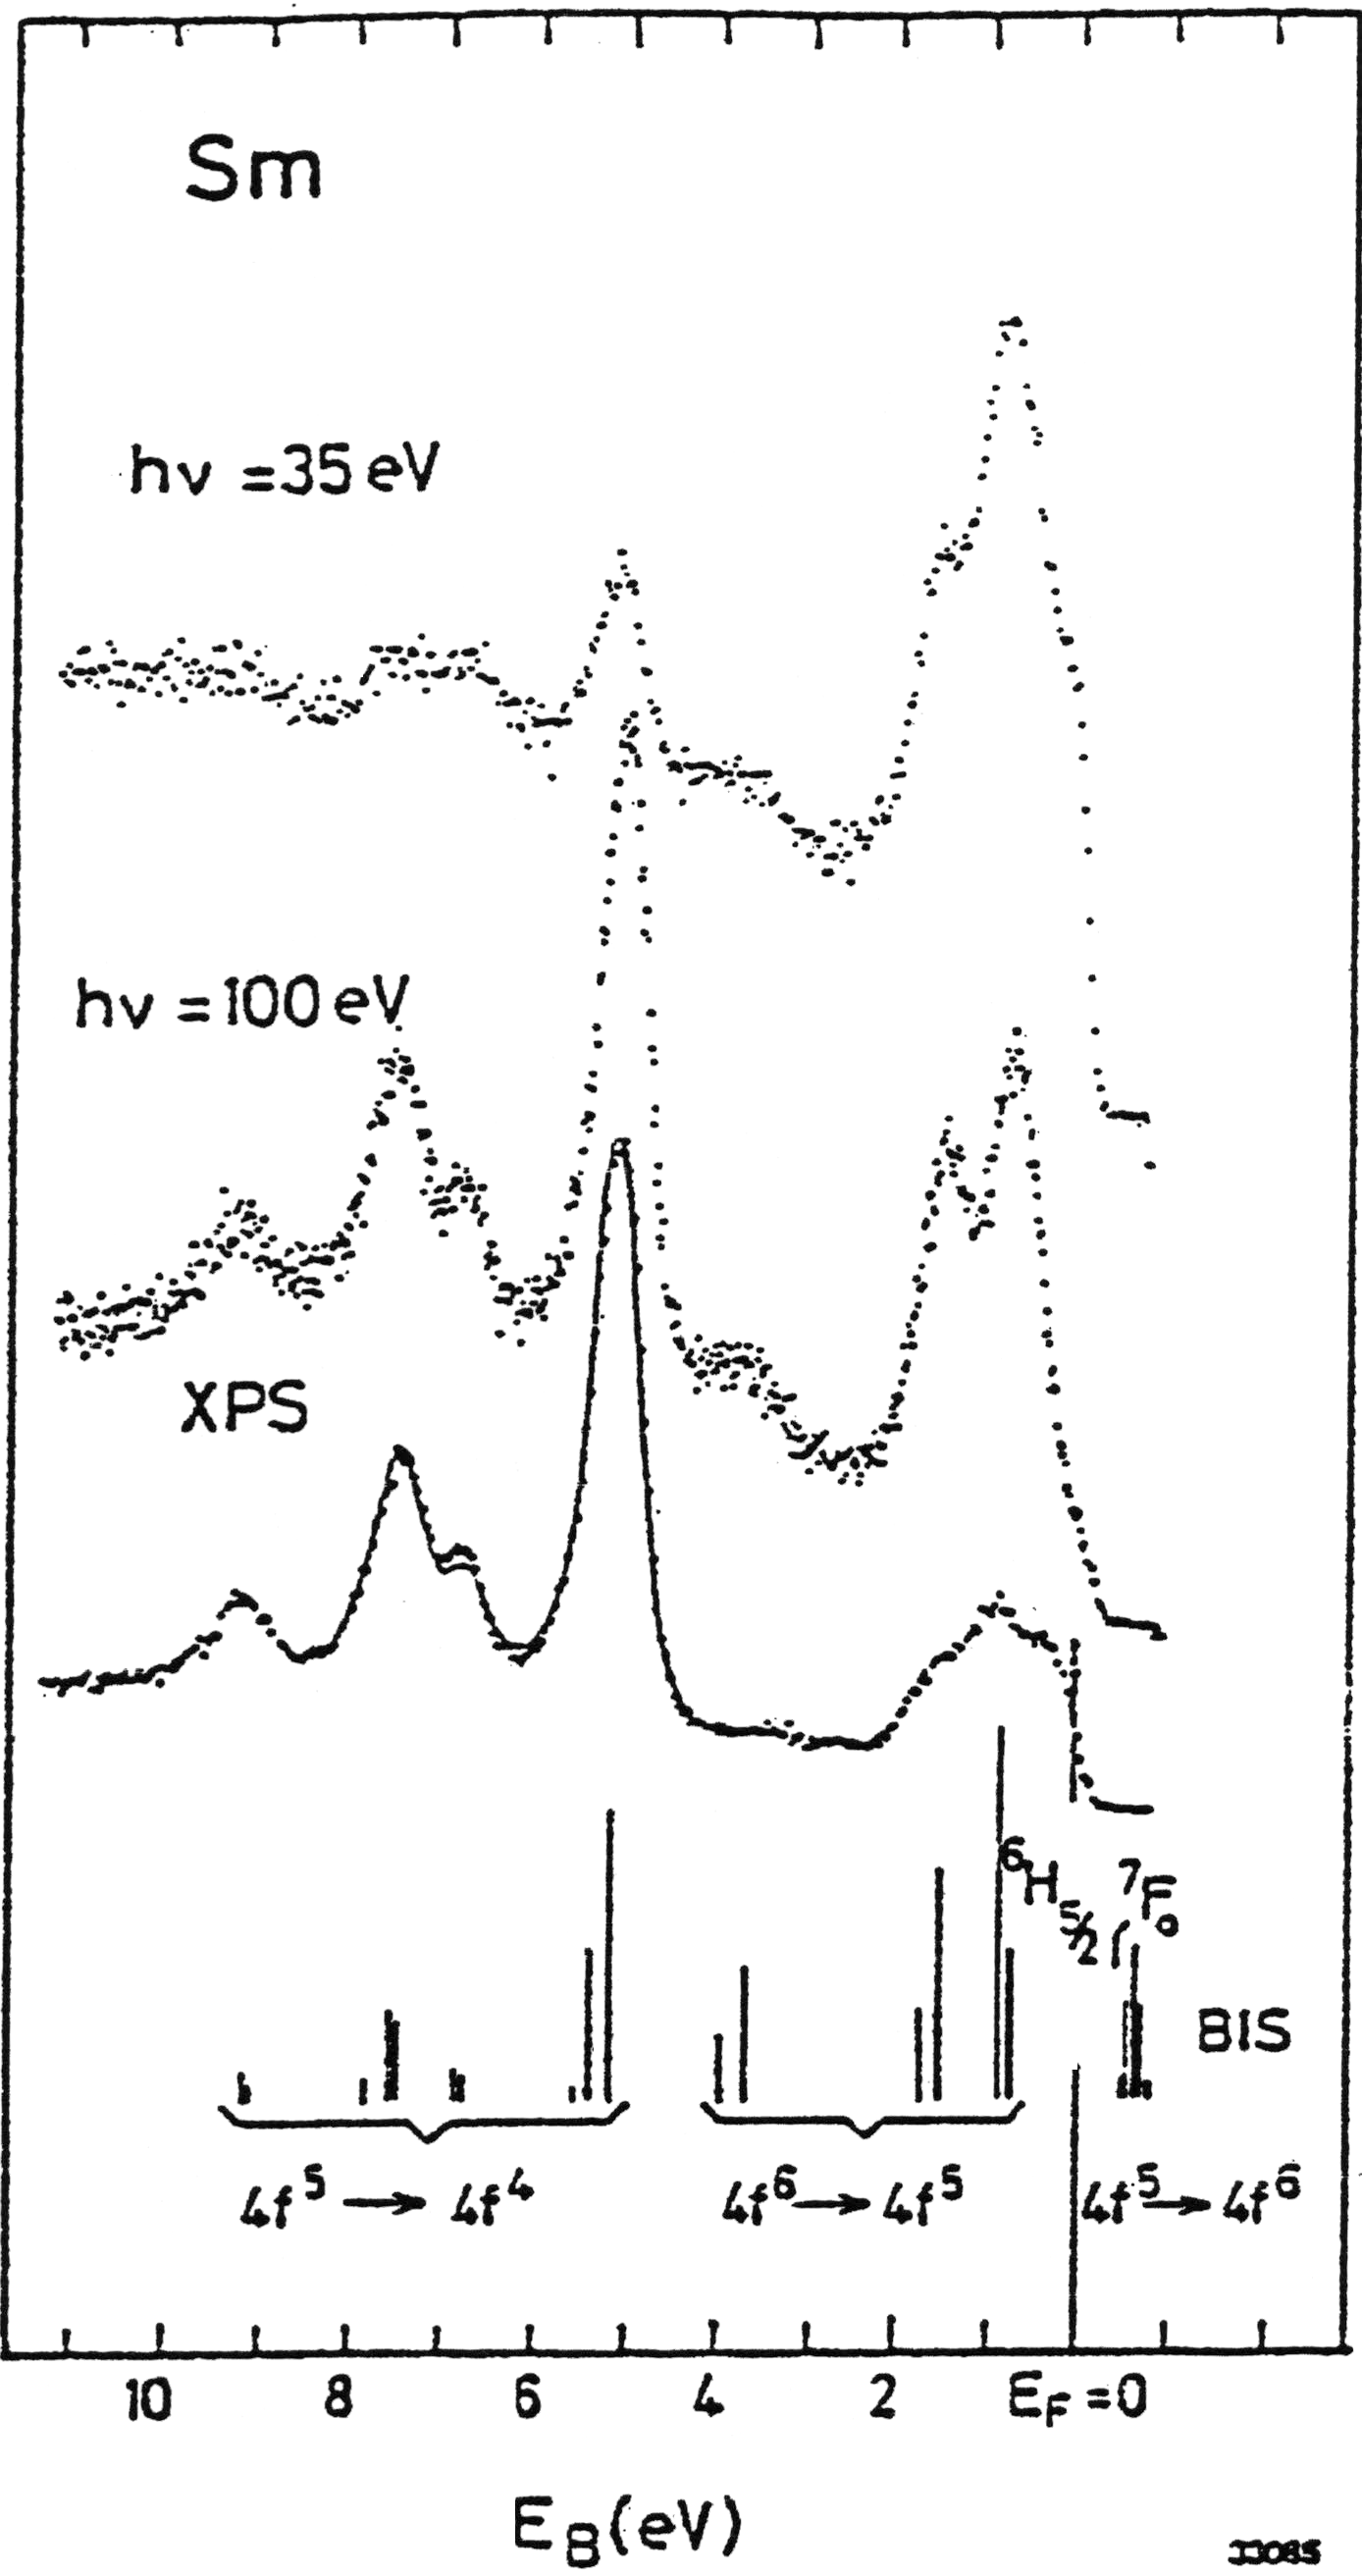
\includegraphics[width=0.7\textwidth]{figures/04_25.png}
	\caption{Synchrotron and XPS spectra of pure samarium \cite{gerken}.}
	\label{fig:smxps}
	\end{center}
\end{figure}

\begin{figure}[h!]
	\begin{center}
	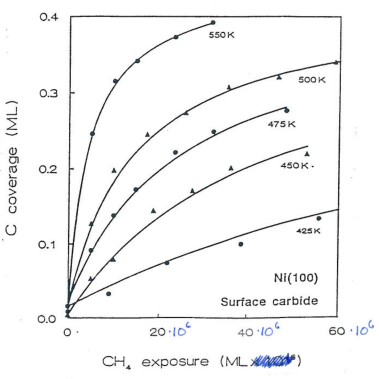
\includegraphics[scale=4]{figures/04_26}
	\caption{Carbon coverage on Ni(100) as a function of methane dosage at various temperatures \cite{chorkendorff2}.}
	\label{fig:ccoverage}
	\end{center}
\end{figure}
